\section{Motivations}
\label{sec:chapter1-motivations}
Machine-to-Machine communication (M2M), also known as Machine Type Communication (MTC) in 3GPP's terminology, is an emerging technology allowing devices to mutually communicate without (or only limited) human intervention. It is expected to become more popular in the next decade and be an integrated part of future wireless networks~\cite{3GPP/service-requirement}\cite{3GPP/ranimprovements}. As an example, Ericsson estimates that $50$ billion MTC devices will be connected to wireless networks by $2020$, among which $2$ billion will be served by cellular networks~\cite{Eri11}.

In opposite to the traditional Human-to-Human (H2H) or Human Type Communication (HTC), MTC presents lots of its own special characteristics. These features are uplink-centric applications, short but more frequent transmission, large number of devices, difficulty to change battery and so on~\cite{FirstLook12}. The aforementioned characteristics pose problems for current deployed wireless systems to handle the traffic from MTC. For example, large number of deployed devices can quickly congest the radio access network, leading to high collision and retransmission rate and low energy efficiency. However, theses devices usually has no power supply and cannot be easily replaced with new battery. Hence, 
how to efficiency support huge amount of devices, namely energy efficiency,  is of a paramount concern for the mobile network operators. It is 
deemed as a key performance indicator that determines if MTC is accepted as a promising technology~\cite{lu11GRS}\cite{Costa14}. 

Nowadays, the research efforts to tackle with MTC traffic in the future wireless networks, can be broadly classified into two categories: \begin{itemize}[leftmargin=*, noitemsep]
	\item Design from scratch of M2M-dedicated wide area networks, i.e., the emerging Low Power Wide Area Network (LPWAN). A representative example is the LoRaWAN~\cite{lora/specification} proposed by LoRa Alliance~\cite{lora_alliance};
	\item Evolution from existing wireless networks, which consists in adapting 3GPP cellular networks to support MTC traffic in addition to H2H traffic, for example the LTE-M~\cite{ratasuk2014narrowband}.
\end{itemize}
According to Cisco's forecast~\cite{cisco2017forecast}, LPWA\footnote{The abbreviations LPWA and LPWAN are interchangeably used in this thesis} and evolved 3GPP networks will have a dominant role for handling MTC traffic in future. It is expected that $29\%$ of MTC devices will be served by LPWA networks and $71\%$ of M2M connections will be served by 3GPP networks (including 2G/3G/4G, shown in Fig.~\ref{fig:m2m-evolution-trend}). Actually, both solutions have their own advantages and shortcoming. 3GPP cellular networks, compared with LPWA networks, have ubiquitous coverage, largely deployed infrastructure, mature user subscription/management system and so on, but they are not easy to be adapted to handle MTC due to compatibility to the H2H. LPWA networks are designed for MTC and thus energy efficient compared with cellular networks, but need huge investment to deploy the dedicated MTC infrastructure. Both types of networks will coexist for a long term.
\begin{figure}[h]
	\centering
	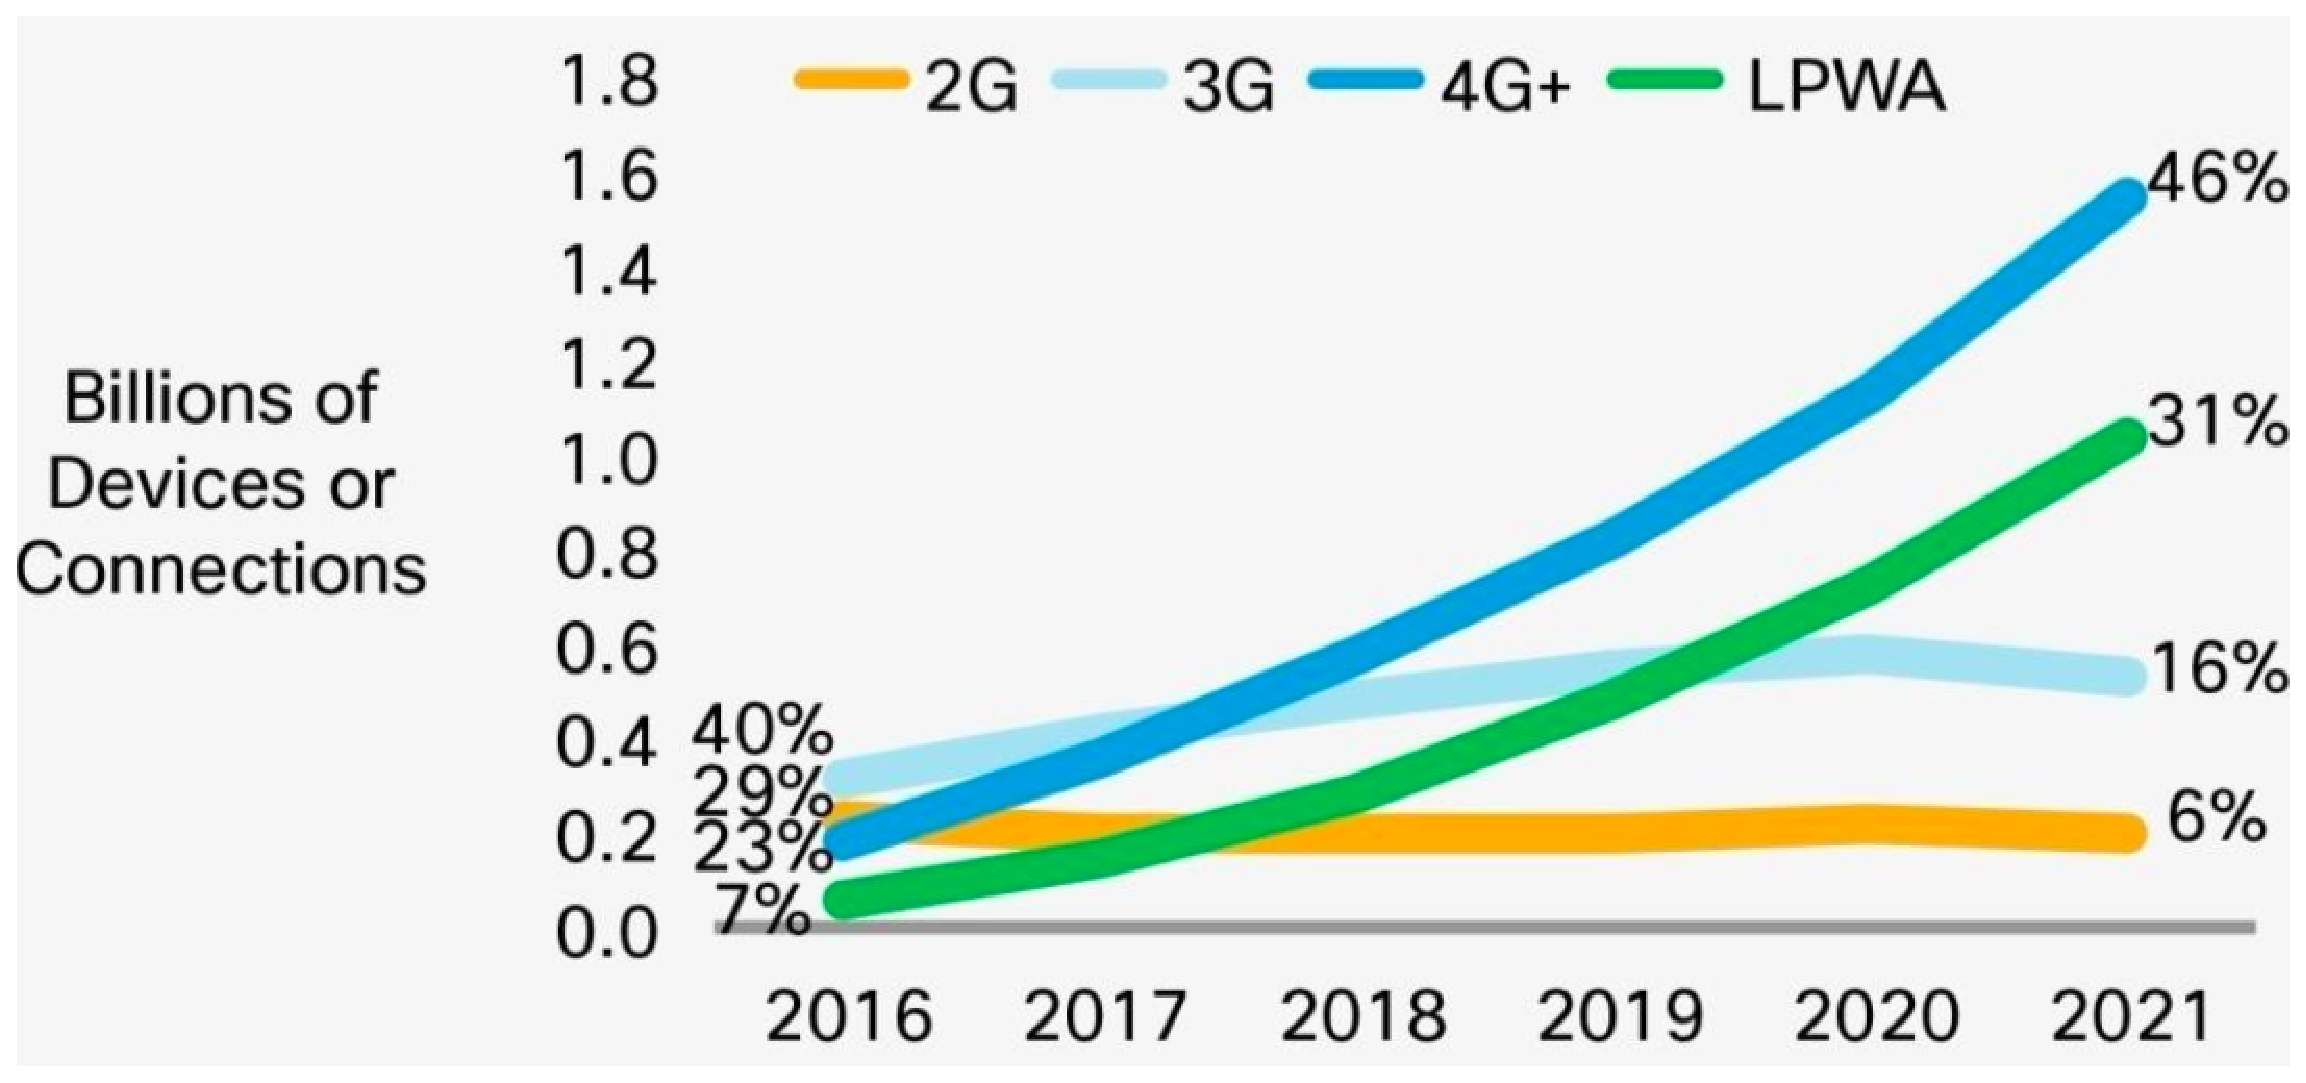
\includegraphics[width=0.8\linewidth]{Chapter1/Figures/Global_Mobile_M2M_Connections.eps}
	\caption{Global Mobile M2M Connections by 2G, 3G, 4G+ and LPWA. Source:~\cite{cisco2017forecast}}
	\label{fig:m2m-evolution-trend}
\end{figure}

In many applications, saving energy for machines is more important than increasing the throughput because machine usually transmit small data but have limited electric energy \cite{YuanHo12}. The energy efficiency is deemed as a key performance indicator that determines if M2M communication is accepted as a promising communication technology~\cite{lu11GRS}. One of important requirements in cellular M2M system is extremely low power consumption~\cite{IEEE/802.16p/10/0002r7}. The hard QoS guarantee is deemed as one of the most important requirement since disasters occur if timing constraints are violated for some MTC applications~\cite{SYLien11}. Energy efficiency is the key in M2M communications, since machine devices are generally powered by batteries~\cite{Costa14}. A critical issue in M2M communications is the energy efficiency as typically the machine devices are powered by batteries of low capacity and thus, it is the key to optimize their consumption \cite{Costa14}.

It should be noted that energy efficiency actually covers device side and network side. For cellular M2M, the network side energy efficiency is not a principal constraint, hence it is out of the scope of this thesis. If not precised, all the energy efficiency we talk about in this thesis is at the device side of the radio access networks.

As one indispensable step to design energy efficiency wireless system (cellular or LWPAN type) for the future M2M application, it is necessary and important to establish appropriate analytical models, which allows to evaluate the performance of radio access networks. From proposed analytical models, we can adjust system parameters to optimize networks based on the characteristics of M2M and get some fundamental design guidelines. Besides performance analysis work, we also consider how to adapt LTE/LTE-A to support MTC. This is the motivation of our work.








